\documentclass[11pt,a4paper]{article}
\usepackage[a4paper,hmargin=1in,vmargin=1in]{geometry}
\usepackage{pgfplots}
\pgfplotsset{compat=1.17}

\usepackage[czech]{babel}
\usepackage[utf8]{inputenc}
\usepackage[T1]{fontenc}

\usepackage{stddoc}
\usepackage{lipsum}
\usepackage{subcaption}

\newcommand{\plus}{{\texttt{+}}}
\renewcommand{\Re}{\operatorname{Re}}
\renewcommand{\Im}{\operatorname{Im}}
\newcommand{\fourier}[3]{\mathcal{F}_{#1}\!\left[#2\right]\!\left(#3\right)}
\newcommand{\ifourier}[3]{\mathcal{F}^{-1}_{#1}\!\left[#2\right]\!\left(#3\right)}


\begin{document}

\pagenumbering{arabic}

% Header
\begin{center}
    {\LARGE\textbf{Laboratorní úloha č. 4}}\\[3mm]
    \begin{minipage}{0.4\textwidth}
        \begin{flushleft}
            \textsc{\today}
        \end{flushleft}
    \end{minipage}
    ~
    \begin{minipage}{0.4\textwidth}
        \begin{flushright}
            \textsc{Martin Šimák}
        \end{flushright}
    \end{minipage}
    \noindent\rule{14.5cm}{0.4pt}
\end{center}

\paragraph*{Měření velkosignálových vlastností mikrovlnných směšovačů a násobičů} Laboratorní úloha poskytuje představu o parametrech a vlastnostech mikrovlnných směšovačů a násobičů a metodice jejich měření pomocí spektrálního analyzátoru a generátorů.

\subsection*{Úkoly měření}
\begin{enumerate}
    \item Závislost konverzních ztrát a izolace LO-IF směšovače na výkonu LO
    \item Bod zahrazení IP3 směšovače
    \item Potlačení zrcadlového kmitočtu směšovače
    \item Konverzní ztráty a harmonické složky násobičů
\end{enumerate}

\subsection*{Použité přístroje a komponenty}
\begin{itemize}
    \item Spektrální analyzátor Agilent E4440A (3~Hz až 26,5~GHz)
    \item Generátor R\&S SMF 100A (1~GHz až 43,5~GHz)
    \item Generátor Agilent E8257D (250~kHz až 50~GHz)
    \item Generátor ELSY SG3000 (100~kHz až 3~GHz)
    \item Koaxiální dolní propust Mini-Circuits VLF-1500\plus~(0~MHz až 1,5~GHz)
    \item Koaxiální dolní propust Mini-Circuits VLF-1800\plus~(0~MHz až 1,8~GHz)
    \item Dělič výkonu/slučovač Mini-Circuits ZX10-2-20-S\plus~(200~MHz až 2~GHz)
    \item Propojovací SMA a BNC kabely
\end{itemize}

\subsection*{Měřené komponenty}
\begin{itemize}
    \item Směšovač Mini-Circuits SYM-30DLHW
    \item Směšovač Mini-Circuits JCIR-152H\plus
    \item Násobič Mini-Circuits ZX90-2-19\plus
    \item Násobič Mini-Circuits ZX90-3-452\plus
\end{itemize}

\subsection*{Popis měření}
\paragraph*{Nastavení přístrojů před měřením} Jako první krok je třeba vyresetovat nastavení genetátorů a spektrálního analyzátoru. U generátoru ELSY tak provedeme deaktivací FM modulace výstupního signálu, u ostatních přístrojů tlačítkem \emph{PRESET}. Jak je vidět ze schématu zapojení na obrázku~\ref{fig:task0-zapojeni}, všechny generátory jsou spojeny se spektrálním analyzátorem BNC kabely přenášejícími referenční 10MHz signál ze spektrálního analyzátoru. Dále je třeba tedy nastavit, aby generátory braly tento externí signál jako svou referenci. Také lze s výhodou zapnout korekci měřeného výkonu na spektrálním analyzátoru o útlum použitého kabelu Pasternack PE300-12.

Generátor R\&S slouží jako zdroj LO, generátor Agilent jako RF1 a generátor ELSY jako RF2. Oba generátory RF jsou spojeny pomocí slučovače RPS-2-30\plus~a na jeho výstupu je dolní propust VLF-1800\plus. Na výstupu generátoru LO je dolní propust VLF-1500\plus. Filtry mají zajistit potlačení vyšších harmonických složek z generátorů.
\begin{figure}[!ht]
    \centering
    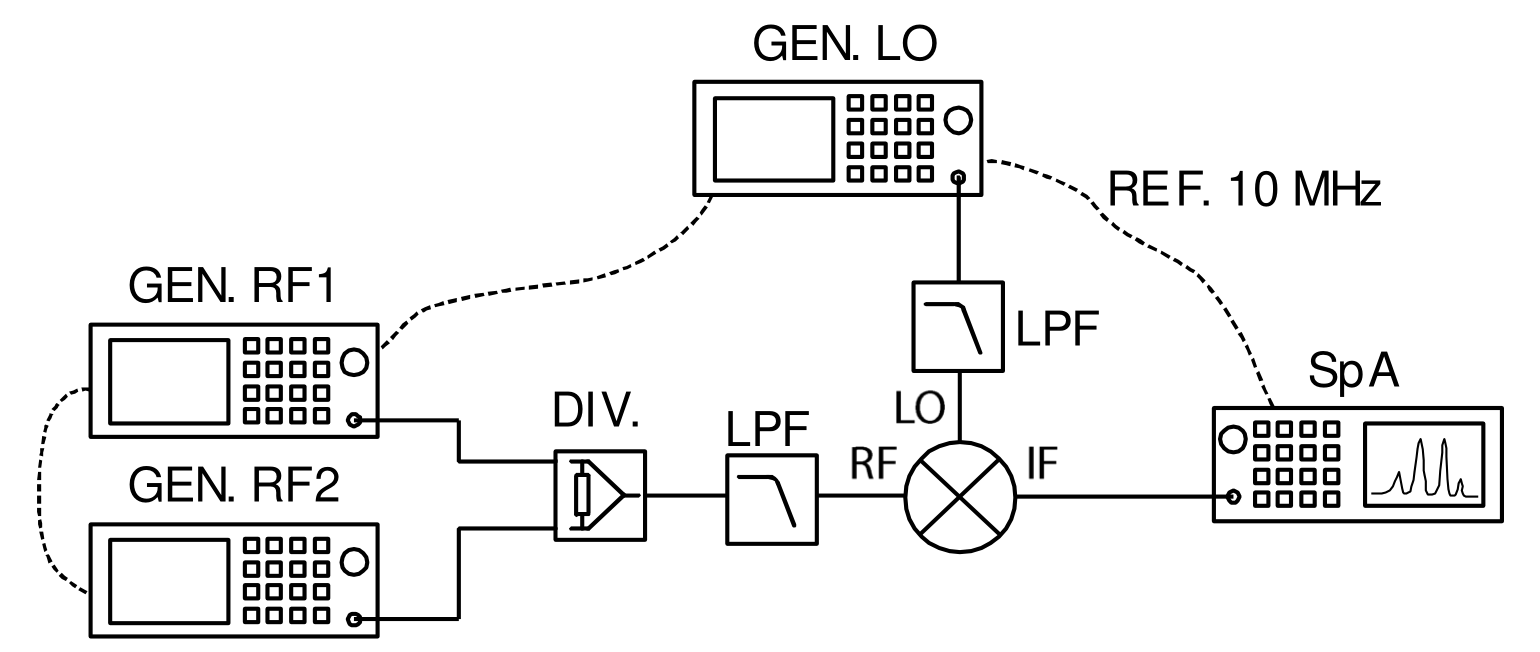
\includegraphics[width=.65\textwidth]{src/task0-zapojeni.png}
    \caption{Schéma zapojení}
    \label{fig:task0-zapojeni}
\end{figure}

% Task 1
\paragraph*{Závislost konverzních ztrát a izolace LO-IF směšovače na výkonu LO} Schéma úlohy zůstává stejné (obrázek~\ref{fig:task0-zapojeni}), přičemž generátor RF2 je vypnutý a měřený směšovač je Mini-Circuits SYM-30DLHW. Nastavení přístrojů:
\begin{itemize}
    \item frekvence generátoru LO 1,2~GHz,
    \item frekvence generátoru RF1 1,1~GHz a výstupní výkon -10~dBm,
    \item referenční výkon spektrálního analyzátoru 0 dBm, rozsah frekvencí do 5~GHz.
\end{itemize}
Za rozmítání výkonu LO v rozsahu -10~dBm až 10~dBm pomocí markerů odečítáme výkon $P_{\mathrm{IF}}$ mezifrekvenčního signálu na $f_{\mathrm{IF}} = 100 \ \mathrm{MHz}$ a výkon $P_{\mathrm{IFLO}}$ prosakujícího signálu LO. Ze změřených hodnot zanesených v tabulce~\ref{table:task1-data} lze následně spočítat konverzní ztráty směšovače $L_{\mathrm c}$ jako rozdíl mezi výkonem -10~dBm vstupního RF signálu a hodnotami $P_{\mathrm{IF}}$ výstupního IF signálu. Dále také výkonový odstup $O_{\mathrm{IFLO}}$ mezifrekvenčního signálu od parazitního LO signálu.
\begin{table}[!ht]
    \centering
    \begin{tabular}{| l || c | c | c | c | c | c | c | c | c | c | c |}
        \hline
        $P_{\mathrm{LO}}$ & -10 & -8 & -6 & -4 & -2 & 0 & 2 & 4 & 6 & 8 & 10\\
        \hline
        $P_{\mathrm{IF}}$ & -64 & -60 & -55 & -49,3 & -42,4 & -35,3 & -29,2 & -24,9 & -22,6 & -21,5 & -21\\
        \hline
        $P_{\mathrm{IFLO}}$ & -37,4 & -35,4 & -33,4 & -31,6 & -29,7 & -28 & -26,7 & -26 & -26,1 & -27,1 & -28,5\\
        \hline\hline
        $L_{\mathrm{c}}$ & 54 & 50 & 45 & 39,3 & 32,4 & 25,3 & 19,2 & 14,9 & 12,6 & 11,5 & 11\\
        \hline
        $O_{\mathrm{IFLO}}$ & -26,6 & -24,6 & -21,6 & -17,7 & -12,7 & -7,3 & -2,5 & 1,1 & 3,5 & 5,6 & 7,5\\
        \hline
    \end{tabular}
    \caption{Naměřené hodnoty výkonů v dBm a zjištěné konverzní ztráty a odstup v dB}
    \label{table:task1-data}
\end{table}

% Task 2
\paragraph*{Bod zahrazení IP3 směšovače} Schéma zapojení i měřený směšovač jsou ponechány z předchozí úlohy s tim, že tentokrát budeme mít zapnuté oba generátory vstupního signálu, čímž simulujeme příjem rádiových signálů rozmístěných v sousedních kanálech po 10~MHz. Nastavení generátorů:
\begin{itemize}
    \item signál LO na hladině 10~dBm a frekvenci 1,2~GHz,
    \item frekvence generátoru RF1 1,1~GHz,
    \item frekvence generátoru RF2 1,11~GHz.
\end{itemize}
Jako poslední krok na spektrálním analyzátoru nastavíme výkon obou RF signálů na -10~dBm a hodnotu RBW tak, aby byly měřitelné výkony $P_3$ intermodulačních produktů 3. řádu na frekvenci
\begin{align*}
    f_3 \in \{80,110\} = \{f_{\mathrm{LO}} - (2f_{\mathrm{RF2}} - f_{\mathrm{RF1}}), f_{\mathrm{LO}} - (2f_{\mathrm{RF1}} - f_{\mathrm{RF2}})\},
\end{align*}
přičemž pro měření jsme zaznamenali vždy významnější ze spektrálních čar. V tabulce~\ref{table:task2-data} jsou také zaneseny naměřené hodnoty výkonů $P_{\mathrm{IF}}$ mezifrekvenčního signálu na frekvenci $f_{\mathrm{IF}} = 100 \ \mathrm{MHz}$ a vypočítaný odstup $O_{\mathrm{IF3}}$ mezifrekvenčního signálu od intermodulačních produktů 3. řádu.
\begin{table}[!ht]
    \centering
    \begin{tabular}{| l || c | c | c | c | c | c |}
        \hline
        $P_{\mathrm{RF}} \ [\mathrm{dBm}]$ & -10 & -8 & -6 & -4 & -2 & 0\\
        \hline
        $P_{\mathrm{IF}} \ [\mathrm{dBm}]$ & -20,5 & -18,4 & -16,4 & -14,4 & -12,4 & -10,4\\
        \hline
        $P_3 \ [\mathrm{dBm}]$ & -85 & -80 & -75 & -70 & -66 & -64\\
        \hline\hline
        $O_{\mathrm{IF3}} \ [\mathrm{dB}]$ & 64,5 & 61,6 & 58,6 & 55,6 & 53,6 & 53,6\\
        \hline
    \end{tabular}
    \caption{Naměřené hodnoty výkonů a zjištěný odstup mezifrekvenčního signálu}
    \label{table:task2-data}
\end{table}

\subparagraph*{Úkol} \emph{Zjistěte bod zahrazení IP3 vztažený k RF vstupu směšovače.} Trend intermodulačního produktu je graficky znázorněn na obrázku~\ref{fig:task2-ip3} a pro bod zahrazení IP3 platí, že $P_{\mathrm{IP3}} = 26,3~\mathrm{dBm}$.
\begin{figure}[!ht]
    \centering
    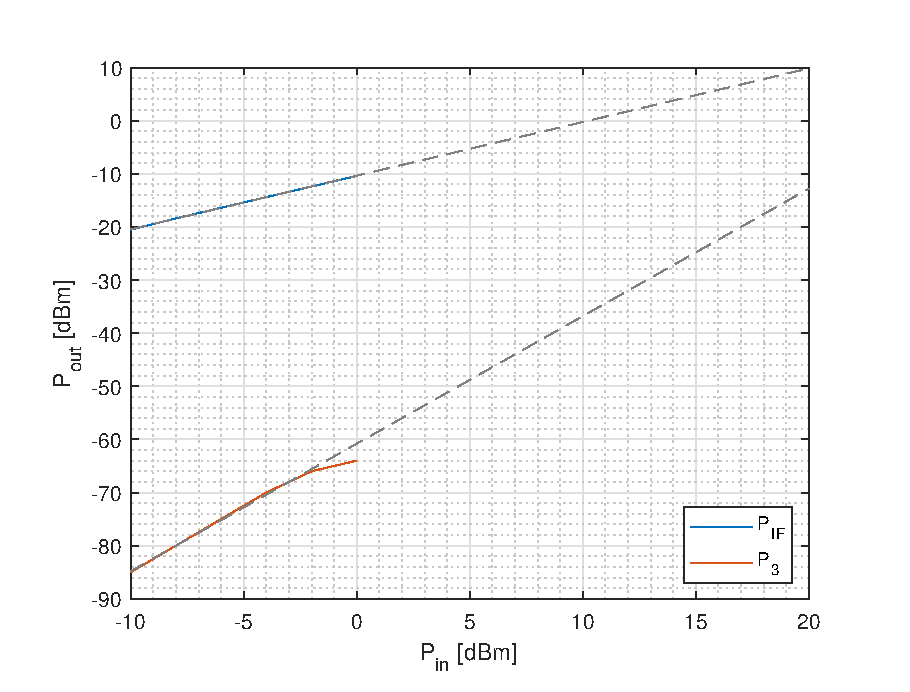
\includegraphics[width=.6\textwidth]{src/task2-ip3.eps}
    \caption{Ilustrace IP3 z naměřených dat}
    \label{fig:task2-ip3}
\end{figure}

% Task 3
\paragraph*{Potlačení zrcadlového kmitočtu směšovače} Schéma zapojení je stejné jako v předchozích dvou úlohách a měřených přístrojem jsou postupně oba uvedené směšovače.

Při použití směšovačů jako \emph{down-converteru} v rádiovém přijímači, kde mezifrekvence $f_{\mathrm{IF}}$ i frekvence LO $f_{\mathrm{LO}}$ jsou pevné, existují dva kmitočty $f_{\mathrm{RF1,2}} = f_{\mathrm{LO}}\pm f_{\mathrm{IF}}$, které po směšování padnou do mezifrekvenčního pásma $f_{\mathrm{IF}}$. Běžné směšovače zrcadlový kmitočet nepotlačují a konverzní ztráty signálů RF1 a RF2 jsou prakticky totožné, pokud je mezifrekvence nízká. Onen nechtěný RF signál je potřeba potlačit buď filtrací, nebo volbou směšovače konstrukčně zabraňujícímu příjmu zrcadlového kmitočtu, nebo ideálně obojím, přičemž při použití směšovače s potlačením zrcadla jsou nároky na následnou filtraci nižší.

Signály RF1 a RF2 nastavíme shodně na -10~dBm, frekvence všech generátorů nastavujeme dle tabulek níže pro jednotlivá měření a výkon LO nastavujeme dle potřeb měřených směšovačů: 10~dBm pro SYM-30DLHW a 18~dBm pro JCIR-152H\plus. Měření spočívá v nastavení správných frekvencí generátorů a následného odečítání hodnot výkonů $P_{\mathrm{IF1}}$ a $P_{\mathrm{IF2}}$ korespondujících \emph{hornímu} a \emph{spodnímu} RF signálu. Jako výsledek dále v tabulkách~\ref{table:task3-data_SYM-30DLHW}~a~\ref{table:task3-data_JCIR-152H+} uvádíme konverzní ztráty $L_{\mathrm L}$ pro spodní signál, konverzní ztráty $L_{\mathrm U}$ pro horní signál a potlačení zrcadlového příjmu $L_{\mathrm M} = L_{\mathrm U} - L_{\mathrm L} = P_{\mathrm{IF1}} - P_{\mathrm{IF2}}$, kde poslední rovnost platí díky naší konfiguraci, kde jsou totožné výkony signálů RF1 a RF2.
\begin{table}[!ht]
    \centering
    \begin{tabular}{| c | c | c || c | c || c | c | c |}
        \hline
        $f_{\mathrm{RF1}}$ & $f_{\mathrm{LO}}$ & $f_{\mathrm{RF2}}$ & $P_{\mathrm{IF1}}$ & $P_{\mathrm{IF2}}$ & $L_{\mathrm{L}}$ & $L_{\mathrm{U}}$ & $L_{\mathrm{M}}$\\
        $[\mathrm{MHz}]$ & $[\mathrm{MHz}]$ & $[\mathrm{MHz}]$ & $[\mathrm{dBm}]$ & $[\mathrm{dBm}]$ & $[\mathrm{dB}]$ & $[\mathrm{dB}]$ & $[\mathrm{dB}]$\\
        \hline\hline
        1000 & 1100 & 1200 & -21,1 & -21,3 & 11,1 & 11,3 & 0,2\\
        \hline
        1100 & 1200 & 1300 & -20,9 & -21,6 & 10,9 & 11,6 & 0,7\\
        \hline
        1200 & 1300 & 1400 & -21,2 & -22,2 & 11,2 & 12,2 & 1\\
        \hline
        1300 & 1400 & 1500 & -21,3 & -23,9 & 11,3 & 13,9 & 2,6\\
        \hline
    \end{tabular}
    \caption{Naměřené hodnoty pro směšovač SYM-30DLHW}
    \label{table:task3-data_SYM-30DLHW}
\end{table}
\begin{table}[!ht]
    \centering
    \begin{tabular}{| c | c | c || c | c || c | c | c |}
        \hline
        $f_{\mathrm{RF1}}$ & $f_{\mathrm{LO}}$ & $f_{\mathrm{RF2}}$ & $P_{\mathrm{IF1}}$ & $P_{\mathrm{IF2}}$ & $L_{\mathrm{L}}$ & $L_{\mathrm{U}}$ & $L_{\mathrm{M}}$\\
        $[\mathrm{MHz}]$ & $[\mathrm{MHz}]$ & $[\mathrm{MHz}]$ & $[\mathrm{dBm}]$ & $[\mathrm{dBm}]$ & $[\mathrm{dB}]$ & $[\mathrm{dB}]$ & $[\mathrm{dB}]$\\
        \hline\hline
        1000 & 1100 & 1200 & -21,6 & -40,9 & 11,6 & 30,9 & 19,3\\
        \hline
        1100 & 1200 & 1300 & -20,8 & -48 & 10,8 & 38 & 27,2\\
        \hline
        1200 & 1300 & 1400 & -21,3 & -42 & 11,3 & 32 & 20,7\\
        \hline
        1300 & 1400 & 1500 & -21,1 & -56,6 & 11,1 & 46,6 & 35,5\\
        \hline
    \end{tabular}
    \caption{Naměřené hodnoty pro směšovač JCIR-152H\plus}
    \label{table:task3-data_JCIR-152H+}
\end{table}

% Task 4
\paragraph*{Konverzní ztráty a harmonické složky násobičů} Schéma zapojení je patrné z obrázku~\ref{fig:task4-zapojeni}. Násobiče jsou nelineární obvody, které na svém výstupu produkují vyšší harmonické složky vstupního signálu. Násobiče bývají optimalizovány tak, aby měly co nejnižší konverzní ztráty pro jednu konkrétní harmonickou složku. Nejběžnější jsou dvojnásobiče až pětinásobiče.
\begin{figure}[!ht]
    \centering
    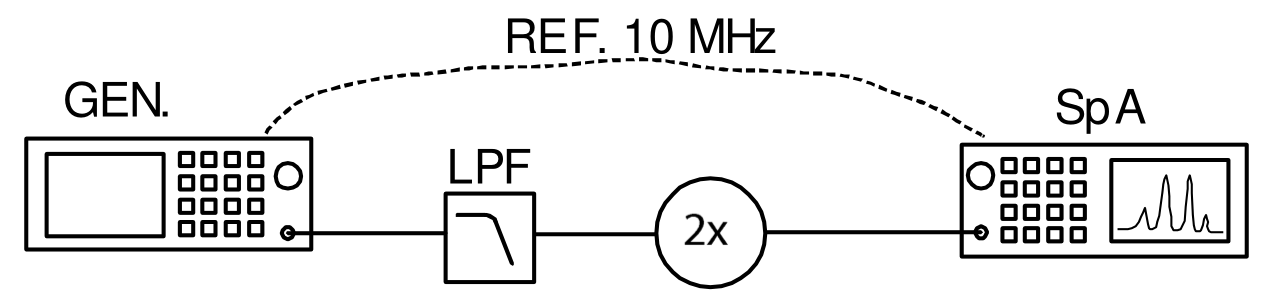
\includegraphics[width=.65\textwidth]{src/task4-zapojeni.png}
    \caption{Schéma zapojení}
    \label{fig:task4-zapojeni}
\end{figure}

Na vstup násobiče připojíme generátor R\&S opět s dolní propustí VLF-1500\plus~pro potlačení vyšších harmonických složek. Frekvence generovaného signálu nechť je $f_1 = 1,2 \ \mathrm{GHz}$. Za rozmítání výkonu vstupního signálu v rozsahu 0~dBm až 10~dBm měříme výkony vyšších harmonických složek na výstupu násobiče. Z naměřených dat lze následně dopočítat konverzní ztráty $L_{\mathrm k}$ a odstup $O_{\mathrm{OUT}}$ výstupního signálu od nejvýkonnější nechtěné harmonické složky. Všechna tato data jsou souhrnně uvedeny v tabulkách~\ref{table:task4-data_ZX90-2-19+}~a~\ref{table:task4-data_ZX90-3-452+}.
\begin{table}[!ht]
    \centering
    \begin{tabular}{| l || c | c | c | c | c | c |}
        \hline
        $P_{\mathrm{IN}} \ [\mathrm{dBm}]$ & 0 & 2 & 4 & 6 & 8 & 10\\
        \hline\hline
        $P_{\mathrm{OUT2}} \ [\mathrm{dBm}]$ & -49,3 & -45,2 & -41,2 & -38,5 & -36,8 & -35,3\\
        \hline
        $P_{\mathrm{OUT3}} \ [\mathrm{dBm}]$ & -49,2 & -47,5 & -45,8 & -43,7 & -43 & -44,2\\
        \hline
        $P_{\mathrm{OUT4}} \ [\mathrm{dBm}]$ & -55,1 & -53,7 & -52,9 & -49,3 & -43,2 & -39,1\\
        \hline\hline
        $L_{\mathrm{k}} \ [\mathrm{dB}]$ & 49,3 & 47,2 & 45,2 & 44,5 & 44,8 & 45,3\\
        \hline
        $O_{\mathrm{OUT}} \ [\mathrm{dBc}]$ & -0,1 & 2,3 & 4,6 & 5,2 & 6,2 & 3,8\\
        \hline
    \end{tabular}
    \caption{Naměřené hodnoty pro násobič ZX90-2-19\plus}
    \label{table:task4-data_ZX90-2-19+}
\end{table}
\begin{table}[!ht]
    \centering
    \begin{tabular}{| l || c | c | c | c | c | c |}
        \hline
        $P_{\mathrm{IN}} \ [\mathrm{dBm}]$ & 0 & 2 & 4 & 6 & 8 & 10\\
        \hline\hline
        $P_{\mathrm{OUT2}} \ [\mathrm{dBm}]$ & -88 & -85 & -85 & -88 & -79 & -71,8\\
        \hline
        $P_{\mathrm{OUT3}} \ [\mathrm{dBm}]$ & -45,6 & -38,7 & -30,8 & -18,6 & -9,8 & -5,1\\
        \hline
        $P_{\mathrm{OUT4}} \ [\mathrm{dBm}]$ & -88 & -88 & -88 & -79 & -79 & -76\\
        \hline\hline
        $L_{\mathrm{k}} \ [\mathrm{dB}]$ & 45,6 & 40,7 & 34,8 & 24,6 & 17,8 & 15,1\\
        \hline
        $O_{\mathrm{OUT}} \ [\mathrm{dBc}]$ & 42.4 & 46.3 & 54.2 & 60.4 & 69.2 & 66.7\\
        \hline
    \end{tabular}
    \caption{Naměřené hodnoty pro násobič ZX90-3-452\plus}
    \label{table:task4-data_ZX90-3-452+}
\end{table}


\subsection*{Závěr}
V rámci laboratorní úlohy jsme si byli schopni udělat představu o parametrech a vlastnostech mikrovlnných směšovačů a násobičů a metodice jejich měření pomocí spektrálního analyzátoru.

Jak je vidět z tabulky~\ref{table:task4-data_ZX90-2-19+}, měření posledního úkolu pro násobič ZX90-2-19\plus~bylo zatíženo chybou, neboť daný násobič by měl mít konverzní ztráty kolem 10~dB. Jinak měření proběhlo bez větších problémů a výsledky odpovídají znalostem nabitým z teoretických přednášek.


\end{document}
